
%%%%%%%%%%%%%%%%%%%%%%%%%%%%%%%%%%%%%%%%%%%%%%%%%%%%%%%%%%%%%%%%%%%%%%%%%
%           Capítulo 3: NOMBRE                   %
%%%%%%%%%%%%%%%%%%%%%%%%%%%%%%%%%%%%%%%%%%%%%%%%%%%%%%%%%%%%%%%%%%%%%%%%%

\chapter{Herramientas Computacionales}
Una vez entendido el funcionamiento detrás los detectores RICH y cómo pueden contribuir a la carcterización de rayos cósmicos, se procederá a explicar en detalle algunas técnicas de análisis de datos, los cuales son utilizados en este trabajo sobre el estudio de los patrones RICH.

\section{Verosimilitud}
La funcíon de verosimilitud se define cómo

\begin{equation}
    L(\theta) = p(x|\theta)
\end{equation}

donde $\theta$ es un conjunto de parámetros característicos de alguna distribución probabilistica e.g. $\sigma$ y $\mu$ para la distribución normal, y x una colección de observaciónes e.g. las posiciones de los fotones cherenkov detectados.\cite{likeCern}\\

 Uno podría interpretar la función de verosimilitud cómo la "probabilidad que una distribución de probabilidad con parámetros $\theta$ representa fielmente el conjunto de datos x."\\

Para aplicar estos métodos a los detectores RICH, se tienen dos formas de atacar el problema; hacer hipótesis globales (una hipótesis única que contempo cada anillo cherenkov en conjunto) o que sean locales (se proponen hipótesis independientes a cada patrón cherenkov) y usar la que proporcione el valor más alto de verosimilitud\cite{Schoning:1997eka}. En este trabajo se utilizó el enfoque local unicamente.\\

\begin{figure}
    \centering
    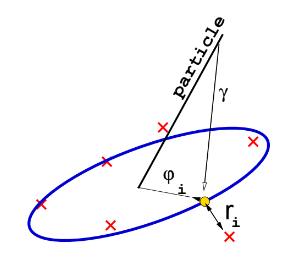
\includegraphics{Tesis-UNAM/Capitulo3/likelihoodAMS.png}
    \caption{Ilustración tomada de \cite{Ypsilantis:2003fs}}
    \label{fig:enter-label}
\end{figure}

La implementación utilizada por el experimento AMS-02 consiste en caracterizar la distribución de los residuales i.e. la distancia de los fotones detectados a la hipotesis\cite{barao2007amsrich, BARAO2003310}, esto debido a que con trigonometría se puede obtener el radio del anillo en función del ángulo cerenkov $r(\theta_c)$ y de la posición del centro del círculo $\phi$.

Por lo que el valor de $\theta_c$ será el obtenido al maximizar la siguiente función de verosimilitud.\cite{barao2007amsrich, BARAO2003310}

\begin{equation}
    L(\theta_c) = \prod_{i=1}^N P_i \left[ r_i(\theta_c, \phi) \right]
\end{equation}

La distribución de probabilidad dependerá de la geometría del detector y de las carcaterísticas del detector

\section{Redes Neuronales}
Las redes neuronales son el andamiaje matemático con el cuál la inteligencia artificial actual esta cimentada, en esta sección se esclarecerá el funcionamiento reduciéndolo a un problema meramente de optimización y se justificará su utilidad.\\

Debido a que las redes neuronales se pueden representar cómo grafos, podemos clasificarlas con base en la topología de su arquitectura, para este trabajo sólo se profundizará las topologías densas y convolucionales.

\subsection{Topología Totalmente Conectada}

\subsubsection{Perceptrón}
\begin{figure}[h!]
    \centering
    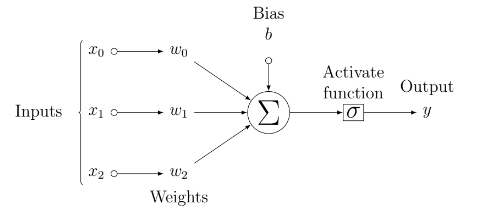
\includegraphics[scale=0.7]{Tesis-UNAM/Capitulo3/perceptron.png}
    \caption{Esquema de un perceptrón}
    \label{fig:enter-label}
\end{figure}

La neurona o perceptrón es la unidad básica de las redes neuronales. A grandes rasgos consta de una función lineal $f:\mathbb{R}^n\xrightarrow{}\mathbb{R}$ compuesta de una función no lineal, i.e. tangente hiperbólica o la función sigmoide.

\begin{equation}
    y = \sigma(w^Tx+b)
\end{equation}

Esta función de activación dota de no-linearidad al perceptrón ya que si apilamos varios perceptrones sin función de activación se obtiene una regresión lineal.\cite{Aggarwal2024DeepLearning} Y también permite constreñir el rango de la función a un intervalo en específico.

\begin{figure}[h!]
    \centering
    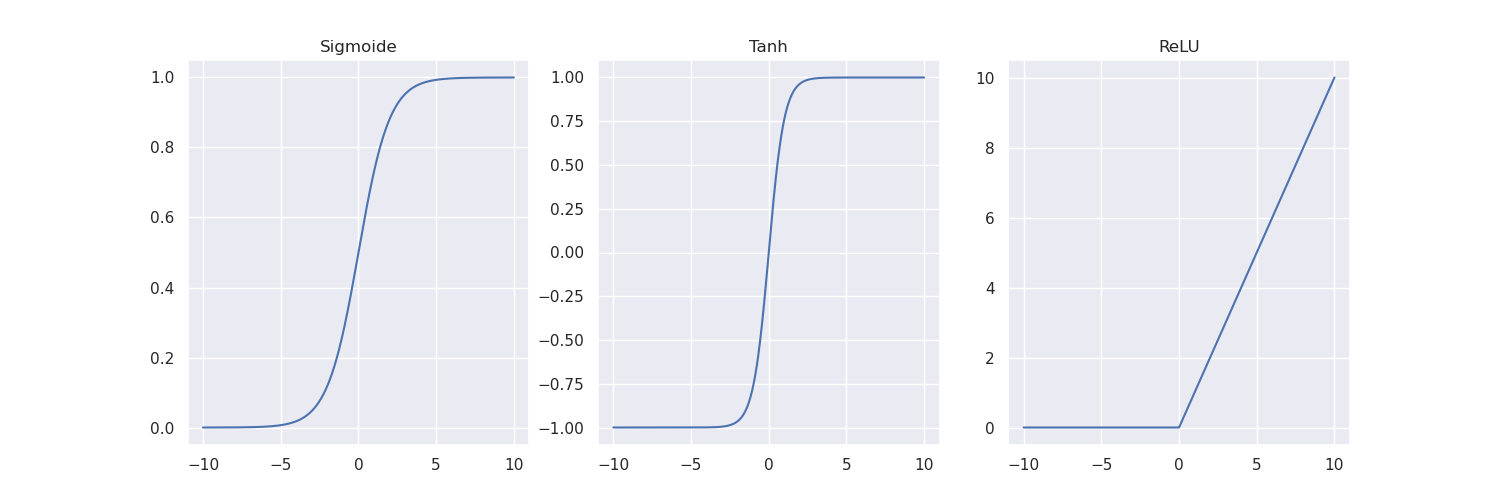
\includegraphics[scale=0.4]{Tesis-UNAM/Capitulo3/Activacion.png}
    \caption{Las funciones de activación más comunes}
    \label{fig:enter-label}
\end{figure}
\subsubsection{Redes Densas}
La razón de por que las redes neuronales son tan utiles para una amplia gama de tareas, es debido a poder apilar varias neuronas, o inclusive conectar varias capas de más de una neurona entre si.\\\\
Se puede demostrar matematicamente que cualquier funcíon se puede aproximar perfectamente con un numero infinito de perceptrones\cite{Aggarwal2024DeepLearning}. Debido a que el coste computacional de tener una infinidad de neurones es enorme, utilizar estas redes sería inmposible. A fortunadamente las redes con miles o inclusive millones de parametros dan muy buenos resultados y gracias a las modernas GPU's se puede entrenar un modelo bastante poderoso en menos de un día\\

Una de las topologías más comunes es conectar todas las neuronas de una capa con todas la neuronas de la siguiente capa.\\

Para este tipo de redes podemos calcular dada una evaluación de una neurona $x^{\left( k-1 \right)}$ de una capa previa con $n_{k-1}$ neuronas, la evaluación de un neurona i de la actual capa $x_i^{\left( k \right)}$ con $n_k$ neuronas mediante la ecuación.\cite{Aggarwal2024DeepLearning, Beyer}

\begin{equation}
    x_i^{\left( k \right)} = \sigma \left( \sum_{j=1}^{n^{\left( k-1 \right)}} w_{ji}^{\left( k \right)}x_j^{\left(k-1 \right)} + b_i^{\left( k\right)}\right) = \sigma(z_i^{(k)})
\end{equation}

\begin{figure}
    \centering
    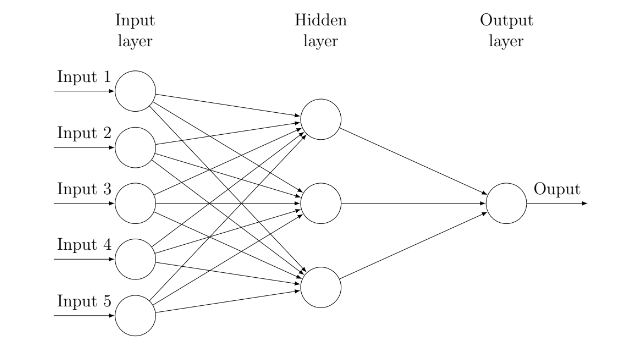
\includegraphics[scale=0.7]{Tesis-UNAM/Capitulo3/Red.png}
    \caption{Red totalmente conectada o densa}
    \label{fig:enter-label}
\end{figure}

\subsubsection{Propagación Hacia Atrás}
La razón por la cual estos modelos se denominan Inteligencia Artificial es debido a la capacidad de corregirse a si mismos y poder por ejemplo, entender un texto, o transcribir un audio sin tener que programar explicitamente todas estas funciones, esto es gracias al algoritmo de propagación hacia atrás.\\

Este algoritmo consiste en modificar los parámetros de la red neuronal con la intención de encontrar el mínimo global de una función error, esto se puede lograr usando el algoritmo de descenso del grádiente ya que el negativo del gradiente apunta en la dirección de descenso más empinado.\\

Para una función $L:\mathbb{R}^n\xrightarrow{} \mathbb{R}$ y una constante $\gamma \in \mathbb{R}^+$ llamada tasa de aprendizaje el algoritmo es el siguiente, rnd se refiere a un punto aleatorio y $\epsilon$ un infinitesimal

\begin{algorithm}
    \caption{Propagación Hacia Atrás}\label{alg:cap}
    \begin{algorithmic}
    \State $\gamma \gets \gamma$
    \State $n_{iter} \gets n_{iter}$
    \State $p_0 \gets rnd$
    \State $tol \gets \epsilon$
    \While{$i<n_{iter}$}
        \State{$p_{i+1} \gets p_{i}-\gamma\nabla L$}
        \If{$d(p_{i+1}, p_{i})>tol$}
        \State $i \gets i+1$
        \EndIf
        \EndWhile
    \end{algorithmic}
\end{algorithm}

Una vez definido el algoritmo tenemos que relacionar el gradiente con los parámetros de la red neuronal, para esto tenemos que derivar el error con respecto a los pesos y posteriormente usar la regla de la cadena \cite{Beyer}

\begin{equation}
    \frac{\partial L}{\partial w_{ij}^{(k)}} = \frac{\partial L}{\partial x_j^{(k)}}\frac{\partial x_j^{(k)}}{\partial z_j^{(k)}}
    \frac{\partial z_j^{(k)}}{\partial w_{ij}^{(k)}}
\end{equation}

Usando la ecuación 3.4 podemos obtener las siguientes relaciones
$$
    \frac{\partial z_j^{(k)}}{\partial w_{ij}^{(k)}} = x_i^{(k-1)}
$$
$$
    \frac{\partial x_j^{(k)}}{\partial z_j^{(k)}} = \sigma'(z_j^{(k)})
$$

Con este algoritmo de propagación atrás podemos hacer de manera iterativa

\begin{equation}
    w_{ij}^{(k)} \xrightarrow{} w_{ij}^{(k)} - \gamma \frac{\partial L}{w_{ij}^{(k)}}
\end{equation}

Actualmente se utilizan diferentes variaciones de este algoritmo pero en principio siguen queriendo obtener un mínimo de una función de error utilizando el descenso del gradiente.\cite{Aggarwal2024DeepLearning, Beyer}

\begin{figure}[h!]
    \centering
    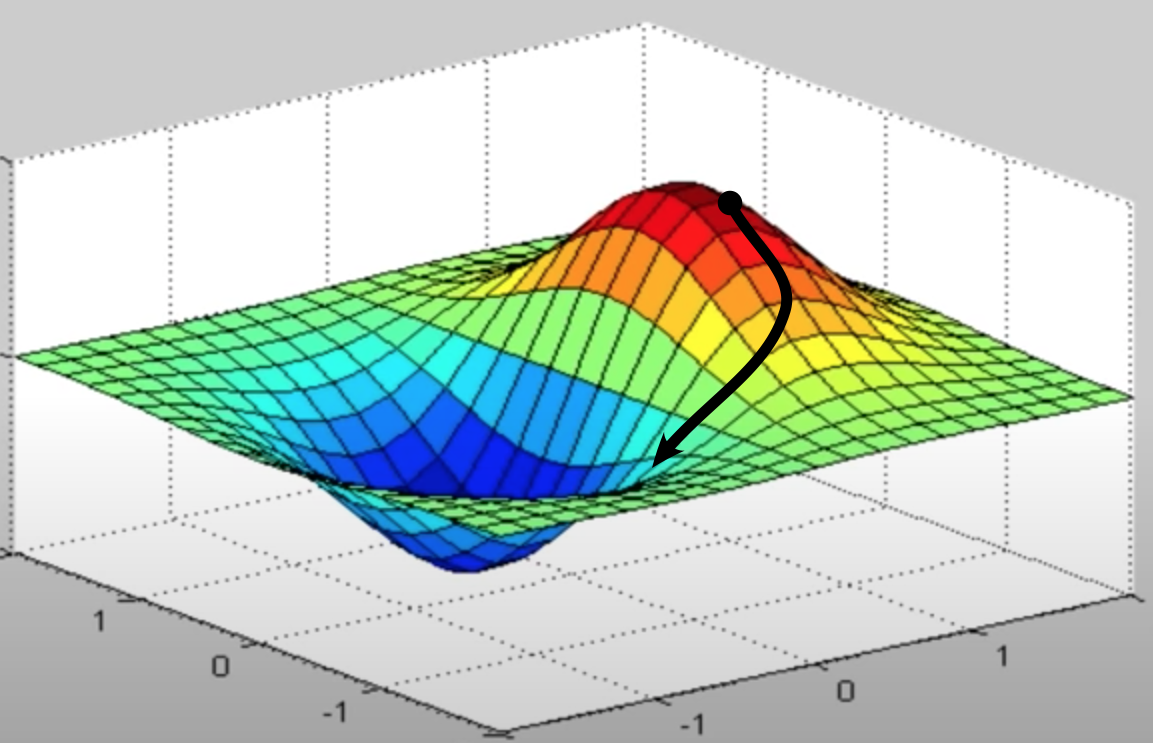
\includegraphics[scale=0.21]{Tesis-UNAM/Capitulo3/gradient.png}
    \caption{Ilustráción gráfica del algoritmo}
    \label{fig:enter-label}
\end{figure}

\subsubsection{Funciones de Error}
El proceso de entrenamiento consiste en disminuir el error de datos previamente ya conocidos proveyendo de retroalimentación al modelo, en este trabjo se utilizó la función de error más común para problemas de regresión, el error promedio al cuadrado\cite{Aggarwal2024DeepLearning}

$$ MSE = \frac{1}{N}\sum_{i=1}^{N}(y-\hat{y})^2$$

y es el valor estimado por el modelo de IA, y $\hat{y}$  es el valor real previamente conocido, esta función es diferenciable pero dominan bastante más los errores grandes.\cite{Beyer}

\subsubsection{Entrenamiento del Módelo}
El entrenamiento del modelo consiste en varias épocas, una epoca es una fase en la cuál todos los datos son utilizados en el entrenamiento, 
y una época consta de diferentes lotes, generalmente son de múltiplos de 8 debido a la arquitectura de las GPU's, y es al final de cada lote que se modifican los parámetros de la red utilizando el algoritmo de propagación hacia atrás.\\

Debido a que se busca prevenir el sobreajuste a los datos de entrenamiento, causando una falla en la predicción de data nueva, se aparta una pequeña parte de los datos para evaluar el modelo al final de cada epoca y corroborar que el error de este lote de validación no seaa mayor al error del entrenamiento (lo que indicaría un sobreajuste del modelo)

\subsection{Toplogía Convolucional}
Las imágenes computacionales se representan en pixeles, en imágenes de blanco y negro el pixel representa varias tonalides grisaceas, esto se puede ver cómo un mapeo del pixel al intervalo $\left[0, 1\right]\in \mathbb{R}$ donde cero representa el blanco y uno el negro. Cuando las imágenes son a color esto se puede hacer de una manera similar, ya que todos los colores se representan con combinaciones de rojo, azul, y verde, así que en este caso el pixel se mapea al subespacio $\left[0, 1\right] \times \left[0, 1\right] \times \left[0, 1\right] \in \mathbb{R}^3$ donde cero representa la ausencia del color en el pixel y uno la saturación total, cada intervalo cerrado necesario para representar la imagen se denomina canal.\\

Por lo tanto las imágenes son matrices, no vectores, ya que un vector no representaria fielmente la localización del pixel con respecto a la imagen, esto hace que querer usar una red densa no sea lo más eficiente y además no sería invariante al desplazamiento\cite{LeCun1998GradientbasedLA}, e.g. si tenemos una esquina, las neuronas que hayan detectado esta esquina sólo podrían identificarla en la misma posición original, no podría detectar la misma esquina en otro lugar de la imagen.\\

\begin{figure}[h!]
    \centering
    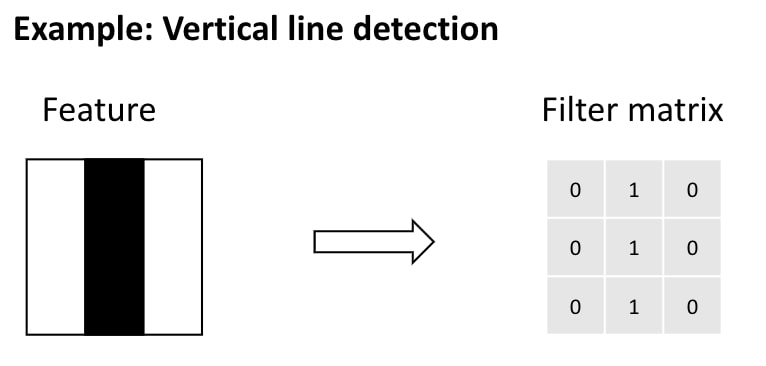
\includegraphics[scale=0.6]{Tesis-UNAM/Capitulo3/filtrosjpeg.jpeg}
    \caption{Filtro capaz de detectar líneas verticales}
    \label{fig:enter-label}
\end{figure}

LeCun en 1998 estudió el árticulo de Hubel y Weisel en donde se descubrió las neuronas del sistema visual de los gatos\cite{LeCun1998GradientbasedLA}, y desarrolló una nueva arquitecura de redes neuronales la cuál denominó convolucional.\\

Esta arquitectura presenta invarianza al desplazamiento al convolucionar filtros sobre toda la imagen. Los filtros son matrices de una dimensión mucho menor a la imagen y que sirven para detectar esquinas, líneas rectas, diagonales, etc... Estos filtros serían los parámetros de la red neuronal a entrenar.\\

\begin{figure}[h!]
    \centering
    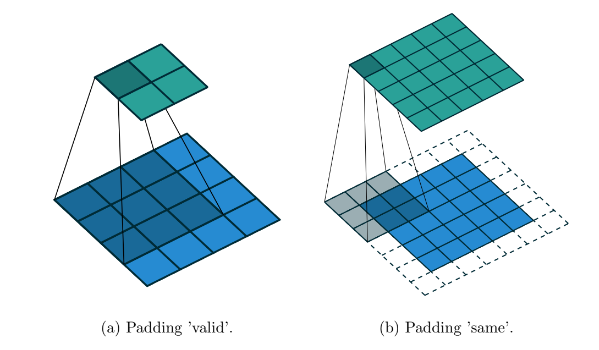
\includegraphics[scale=0.75]{Tesis-UNAM/Capitulo3/padding.png}
    \caption{Los cuadros azules representan la data original y los transparentes los valores añadidos en el padding. \cite{Beyer}}
    \label{fig:enter-label}
\end{figure}

La razón de llamarse redes convolucionales es que estos filtros se convolucionan con la imagen, detectando patrones en la imagen entera y respetando la invarianza al desplazamiento de los mismos.También hay que aclarar que de esta manera se obtiene un rendimiento mucho mayor con un número bastante menor de parametros con respecto a una topología totalmente conectada.\cite{LeCun1998GradientbasedLA}\\

Cómo los anillos cerenkov se pueden representar a blanco y negro, se utilizará sólo un canal. Al realizar la convolución de los filtros con la imagen se obtiene mediante la siguiente ecuación, con k un filtro.\cite{Beyer}

\begin{equation}
    y_{a, b} = \sum_{i=-u}^u\sum_{j=-u}^uk_{i,j}x_{a+i,b+j}+B
\end{equation}

Con a, b los índices del pixel de la imagen, y un tamaño de filtro $f\timesf=(2u+1)\times(2u+1)$ impar, además cada filtro contiene un valor de sezgo B, finalmente a la convolución resultante se le aplíca una función de activación.

\subsubsection{Padding y Striding}
Debido a que la operación convolución puede reducir la dimensionalidad de la imagen, al conectar varias capas convolucional podemos inclusive reducir la imagen a una matriz de un sólo elemento. Una forma de solucionar este problema es incluyendo padding en cada capa convolucional.\\

\begin{figure}[h!]
    \centering
    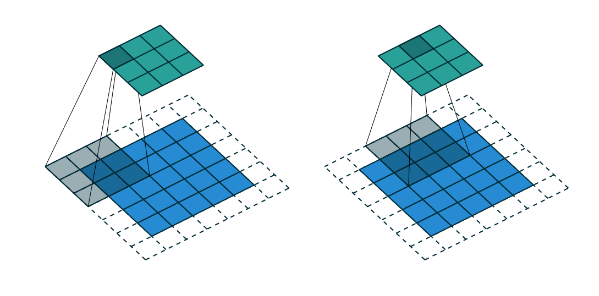
\includegraphics[scale=0.75]{Tesis-UNAM/Capitulo3/stridding.png}
    \caption{Dos convoluciones seguidos con un stridding de 2 en el eje x y padding "same". \cite{Beyer} }
    \label{fig:enter-label}
\end{figure}

Este padding le añade pixeles a la frontera de los datos con ceros u otros valores predichos. Los frameworks de IA más usados contienen opciones predefinidas, cómo "same" que mantiene el tamaño antes de la convolución; o "valid" que añade sólo los valores necesarios para que pueda ser correcta la convolución.\\

También existe el "stridding" lo que define el tamaño del desplazamiento en píxeles durante cada operación de convolución, puede ser uno, o dos píxeles por ejemplo, y también variar el tamaño si el desplazamiento es en el eje x o y, e.g. dos horizontales y uno vertical. Esto puede reducir la dimensión de la data pero hay momentos donde llega a ser beneficioso, por ejemplo si se busca optimizar la velocidad de entrenamiento del modelo, reduciendo el número de parámetros a entrenar conforme se avanza en la red neuronal.\\
